\documentclass[a4paper]{article}
\usepackage[utf8]{inputenc}
\usepackage{float}
\usepackage{enumitem}
\usepackage{caption}
\usepackage[table]{xcolor}    
\usepackage{booktabs}         
\usepackage{longtable}       

\usepackage[margin=20mm]{geometry}
\usepackage{titlesec}
\usepackage{xcolor}
\usepackage{longtable}
\usepackage{graphicx}
\usepackage{advdate}
\usepackage{cmbright}
\usepackage{array}
\usepackage{makecell}


\definecolor{UnipdRed}{RGB}{155, 0, 20}

\usepackage{sectsty}
%\setcounter{secnumdepth}{0}
\allsectionsfont{\sffamily\color{UnipdRed}}


\usepackage{fancyhdr}
\pagestyle{fancy}
\renewcommand{\headrulewidth}{0pt}
\renewcommand{\footrulewidth}{0pt}
\setlength\headheight{80.0pt}
\addtolength{\textheight}{-80.0pt}
\chead{
\includegraphics[width=0.5\columnwidth]{logos/logo-unipd800.pdf}\hspace{0.25\columnwidth} 
\includegraphics[width=0.2\columnwidth]{logos/DEI.pdf}}
\cfoot{}

%\renewcommand{\maketitle}{
%\maketitle
%\thispagestyle{fancy}

%\pagebreak
%\pagestyle{plain}
%\setlength\headheight{20.0pt}
%\addtolength{\textheight}{-20.0pt}
%}

\makeatletter         
\renewcommand\maketitle{
{\raggedright 
\begin{center}

{   
    \Large\bfseries\sffamily 
    \@title}\\[4ex] 
    \Large
    \textbf{Master Degree in Computer Engineering\\
    Master Degree in Cybersecurity\\
    Master Degree in ICT for Internet and Multimedia\\}
    \large
    \vspace{\baselineskip}
    \deadline{24 April}
    \vspace{30mm}
    \centering
\begin{longtable}{|p{.3\columnwidth}|p{.3\columnwidth} |p{.3\columnwidth}|} 
\hline
 \makecell{\textbf{Group Acronym}} & \multicolumn{2}{c|}{\makecell{BAR}} \\ \hline
 \makecell{\textbf{Last Name}} & \makecell{\textbf{First Name}} & \makecell{\textbf{Badge Number}} \\
 \hline
 \makecell{Bruzzese} & \makecell{Fulvio} & \makecell{2180395} \\\hline
 \makecell{Foffano} & \makecell{Claudia} & \makecell{2165805} \\\hline
 \makecell{Halawani} & \makecell{Sondos} & \makecell{2181752} \\\hline
 \makecell{Lacobet} & \makecell{Ecaterina} & \makecell{2190088} \\\hline
 \makecell{Núñez Casal} & \makecell{Luis Ignacio} & \makecell{2185475} \\\hline
\end{longtable}
    \end{center}}
    \thispagestyle{fancy}
    %\thispagestyle{empty}
    \pagebreak
    \pagestyle{plain}
    \setlength\headheight{25.0pt}
    \addtolength{\textheight}{-25.0pt}
}
\makeatother


\newcommand{\hw}{Homework 1 – Server-side Design and Development}


\title{
Web Applications A.Y. \AdvanceDate[-365]\the\year{}-\AdvanceDate[365]\the\year{}\\
\vspace*{0.5\baselineskip}
\hw}

\newcommand{\deadline}[1]{Deadline: #1, \the\year{}} 





\begin{document}
\maketitle



\section{Objectives}
%Brief description of the overall objectives of your system.
%What your system will be used for? Why is it important? What problems does it solve?



The objective of the project, as a continuation of the system developed during the database course, is to design and implement a web interface for managing the data of a lounge bar management system. The project focuses on the interaction between users and the back end, as well as on the correct organization and exchange of information related to customers, staff, drinks, reservations, and orders.

The system is designed to support the main activities of a lounge bar in a structured and efficient manner. In particular, it enables the management of customer reservations, drink orders, table availability, and staff shifts. It also provides basic support for inventory management, as drinks are associated with supplies used in their preparation.

The application supports different categories of users, each with specific permissions and functionalities, ensuring a clear separation of roles and responsibilities. In particular, customers interact with the reservation functionalities, while waiters manage orders and service operations.

Overall, the purpose of the system is to provide a reliable and user-friendly platform that improves the organization of the lounge bar and simplifies the management of its daily operations.




\section{Main Functionalities}
%What are the main functionalities of the web app? what services does it offer and how it is organized?

Lorem ipsum dolor sit amet, consectetur adipiscing elit, sed do eiusmod tempor incididunt ut labore et dolore magna aliqua. Ut enim ad minim veniam, quis nostrud exercitation ullamco laboris nisi ut aliquip ex ea commodo consequat. Duis aute irure dolor in reprehenderit in voluptate velit esse cillum dolore eu fugiat nulla pariatur. Excepteur sint occaecat cupidatat non proident, sunt in culpa qui officia deserunt mollit anim id est laborum.

The web application allows users to interact with the data managed by the lounge bar system and to update such data through dedicated functionalities. \\
The system is organized into three main areas:

\begin{description} [font=\normalfont]
    \item[Public area:] accessible to both unregistered and registered users. This area corresponds to the homepage of the application and provides general information about the lounge bar, together with access to authentication functionalities such as login and registration.

    \item[Customer area:] this area includes the functionalities available to authenticated customers. \\ 
    In particular, customers can:
    \begin{itemize}
        \item create reservations for a specific table, date, time interval, and number of people;
        \item leave a review for a specific waiter with a rating from 1 to 5 and the option to add a comment;
        \item interact with the system by checking the order status for their table.
    \end{itemize}

    \item[Waiter area:] this area is dedicated to staff responsible for service operations. \\
    In particular, waiters can:
    \begin{itemize}
        \item manage customer orders;
        \item add drinks to an order and update its status;
        \item manage and search supplies in stock;
        \item view their assigned shifts and create new ones.
    \end{itemize}
\end{description}



The application in general includes support functionalities related to order handling and basic stock control. Since drinks are associated with supplies through their composition, the system can keep track of ingredient usage and available quantities.

Different users have access to different parts of the application depending on their role. Waiters are responsible for operational tasks: they manage orders, add drinks, update order statuses, and keep track of supplies. Customers can make reservations, leave reviews for waiters, and check the status of their table's order. 

Unregistered users can only see general information about the lounge bar. To access any protected functionality, a user must first create an account and log in. Once logged in, the system determines what the user can see and do based on their role.




\section{Data Logic Layer}
\label{sect:datalogiclayer}

\subsection{Entity-Relationship Schema}
\label{subsec:entity-relational-schema} 
\begin{figure}[H]
    \centering
    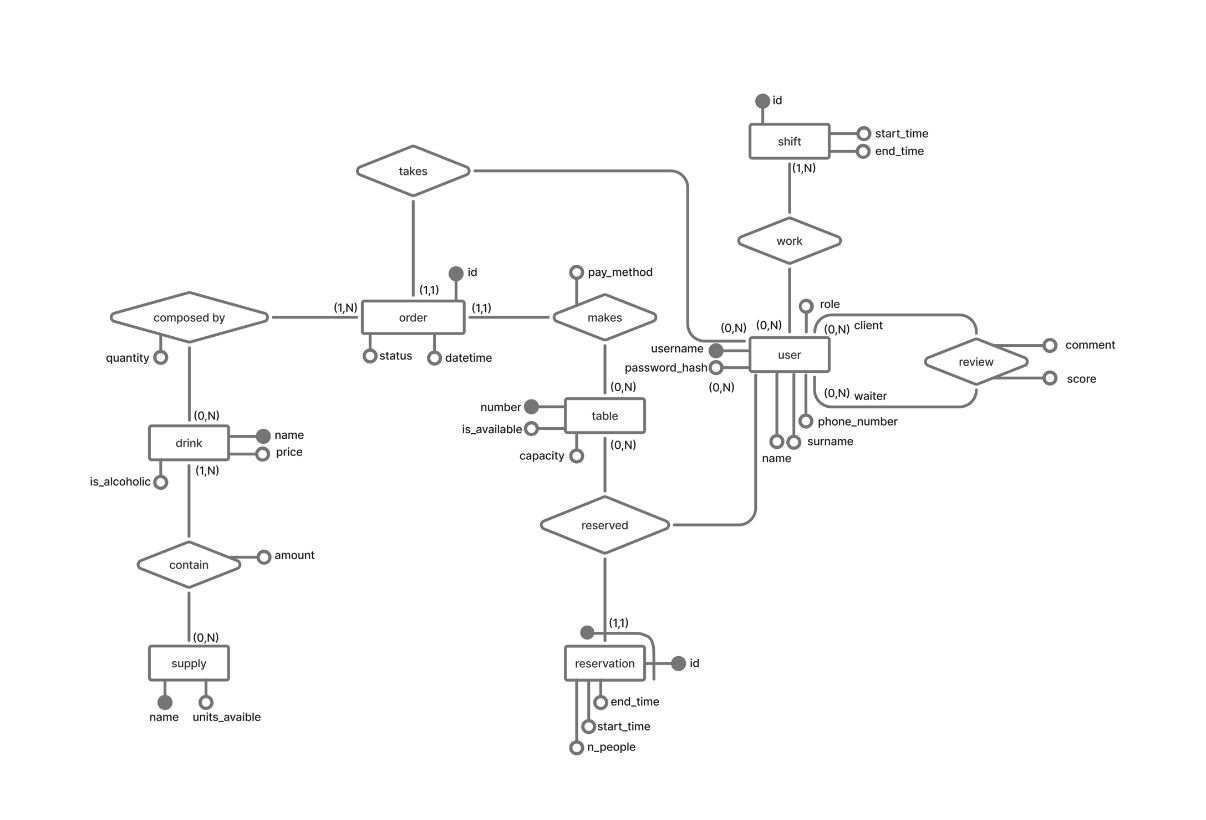
\includegraphics[width=1.1\textwidth]{logos/ER-Schema.jpeg}
    \caption{ER Schema}
\end{figure}

The entity–relationship schema of the Lounge Bar system contains 10 main entities and 3 associative entities used to resolve many-to-many relationships.
The entity–relationship schema models the core operations of a lounge bar management system, including order handling, reservations, staff scheduling, and inventory management. The design ensures consistency and normalization by separating entities and resolving many-to-many relationships through associative entities.

\section{Entites}
\label{sect:entites}

\begin{itemize}
\item
  User\\
  Represents all system users, including both customers and staff
  (waiters).\\
  Each user is uniquely identified by the attribute \emph{username}
  (primary key).\\
  Additional attributes include \emph{password\_hash}, \emph{name},
  \emph{surname}, \emph{phone\_number}, and
  \emph{role}.\\
  The \emph{role} attribute distinguishes between customers and
  employees, allowing role-based interactions within the system.
\item
  Drink\\
  Represents the drinks available in the bar.\\
  Each drink is uniquely identified by \emph{name} (primary key).\\
  Additional attributes include \emph{price} and \emph{is\_alcoholic}.
\item
  Supply\\
  Represents the ingredients or materials used to prepare drinks.\\
  Each supply is uniquely identified by \emph{name} (primary key) and
  includes the attribute \emph{units\_available}, which supports
  inventory management.
\item
  Table\\
  Represents physical tables in the bar.\\
  Each table is uniquely identified by \emph{number} (primary key).\\
  Additional attributes include \emph{capacity} and
  \emph{is\_available}.
\item
  Order\\
  Represents a customer order.\\
  Each order is identified by \emph{id} (primary key).\\
  Attributes include \emph{date\_time}, \emph{status}, and
  \emph{pay\_method}.\\
  Each order is associated with exactly one waiter
  (\emph{user\_waiterID}) and one table (\emph{tableID}), establishing
  two many-to-one relationships.
\item
  Reservation\\
  Represents reservations made by customers.\\
  Each reservation is identified by \emph{id} (primary key).\\
  Attributes include \emph{date}, \emph{start\_time}, \emph{end\_time},
  and \emph{n\_people}.\\
  Each reservation is associated with exactly one customer
  (\emph{user\_customerID}) and one table (\emph{tableNumber}).
\item
  Shift\\
  Represents a working shift.\\
  Each shift is identified by \emph{id} (primary key) and includes
  \emph{shift\_date}, \emph{start\_time}, and \emph{end\_time}.
\item
  Review\\
  Represents feedback provided by customers about waiters.\\
  Each review links a \emph{customer} to a \emph{waiter} and includes
  \emph{score} and \emph{comment}.\\
  This entity models a relationship between two instances of the User
  entity with different roles.
\end{itemize}




\subsection{Relationship Entites (Associative Tables)}
\label{sect:entites}

\begin{itemize}
\item
  Order\_Item\\
  Resolves the many-to-many relationship between Order and Drink.\\
  Each record links one order to one drink and includes the attribute
  \emph{quantity}.\\
  The primary key is composed of (\emph{orderID}, \emph{drink\_name}).
\item
  Composition\\
  Resolves the many-to-many relationship between Drink and Supply.\\
  Each record specifies which supplies are required to prepare a drink
  and in what \emph{amount}.\\
  The primary key is (\emph{drink\_name}, \emph{supply\_name}).
\item
  Work\_Slot\\
  Resolves the many-to-many relationship between User (waiters) and
  Shift.\\
  Each record associates a waiter with a shift.\\
  The primary key is (\emph{shiftID}, \emph{user\_waiterID}).
\end{itemize}








\subsection{Relationships and Cardinalities}


\begin{itemize}
\item
  A User (waiter) can manage multiple Orders, while each order is
  handled by exactly one waiter (1--N).
\item
  A User (customer) can create multiple Reservations, while each
  reservation is associated with exactly one customer (1--N).
\item
  A Table can be associated with multiple Orders and Reservations over
  time, but each order/reservation refers to exactly one table (1--N).
\item
  An Order contains multiple Drinks, modeled through Order\_Item (N--M).
\item
  A Drink is composed of multiple Supplies, modeled through Composition
  (N--M).
\item
  A User (waiter) can work in multiple Shifts, and each shift can
  include multiple waiters (N--M via Work\_Slot).
\item
  A Review represents a relationship where a customer evaluates a
  waiter, allowing multiple reviews per user pair over time.
\end{itemize}





\subsection{Design Considerations}

The schema is normalized to reduce redundancy and ensure data
consistency.\\
Many-to-many relationships are explicitly resolved using associative
entities (Order\_Item, Composition, Work\_Slot), allowing the inclusion
of additional attributes such as quantity and amount.

Foreign keys enforce referential integrity between entities, ensuring
that all relationships remain consistent. For example, orders cannot
exist without a valid waiter and table, and reservations must reference
existing users and tables.

The use of role-based attributes within the User entity avoids
duplication while still supporting different behaviors for customers and
staff.












\section{UI Layout Design and Presentation Logic Layer}

\subsection{Homepage}

The homepage represents the main entry point of the web application. It provides a general overview of the lounge bar system and allows users to easily navigate to the main functionalities of the platform. In particular, it contains a navigation bar with the main sections of the application and a central area presenting a welcome message and a short description of the system.

A prominent action button is included to allow users to quickly access the reservation functionality. Additional navigation options such as viewing the menu, checking availability, and contacting the bar are also provided to enhance usability and user experience.

\begin{figure}[H]
        \centering
    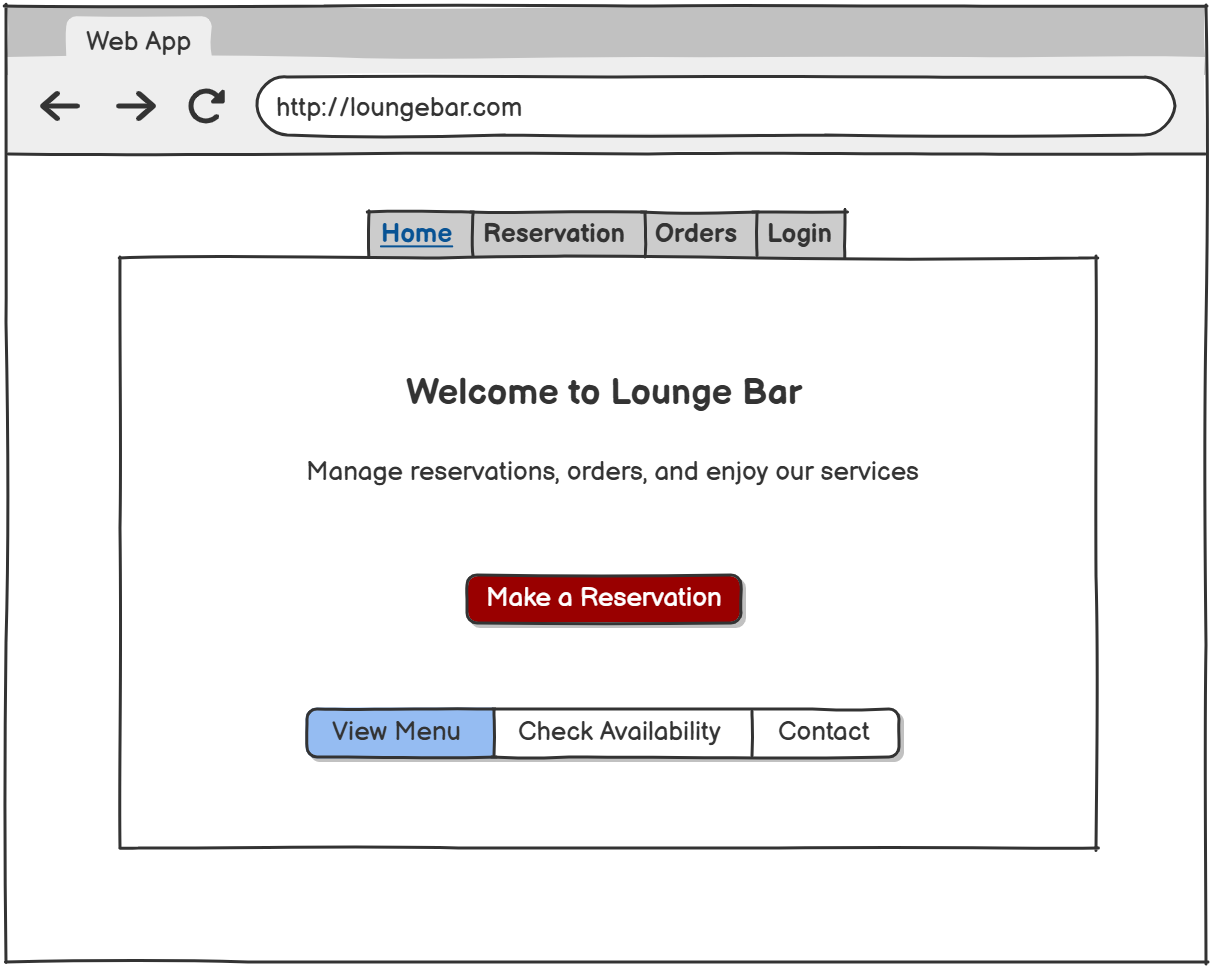
\includegraphics[width=1.1\textwidth]{logos/Home.png}
    \caption{Homepage layout of the Lounge Bar web application}
\end{figure}


\subsection{Login Page}

The login page allows users to authenticate and access the system according to their role. It consists of a simple form containing input fields for username and password. The interface is designed to be minimal and user-friendly, ensuring a straightforward login process.

A link to the registration page is also provided for users who do not yet have an account. Upon successful authentication, users are redirected to the appropriate section of the application based on their role.

\begin{figure}[H]
    \centering
    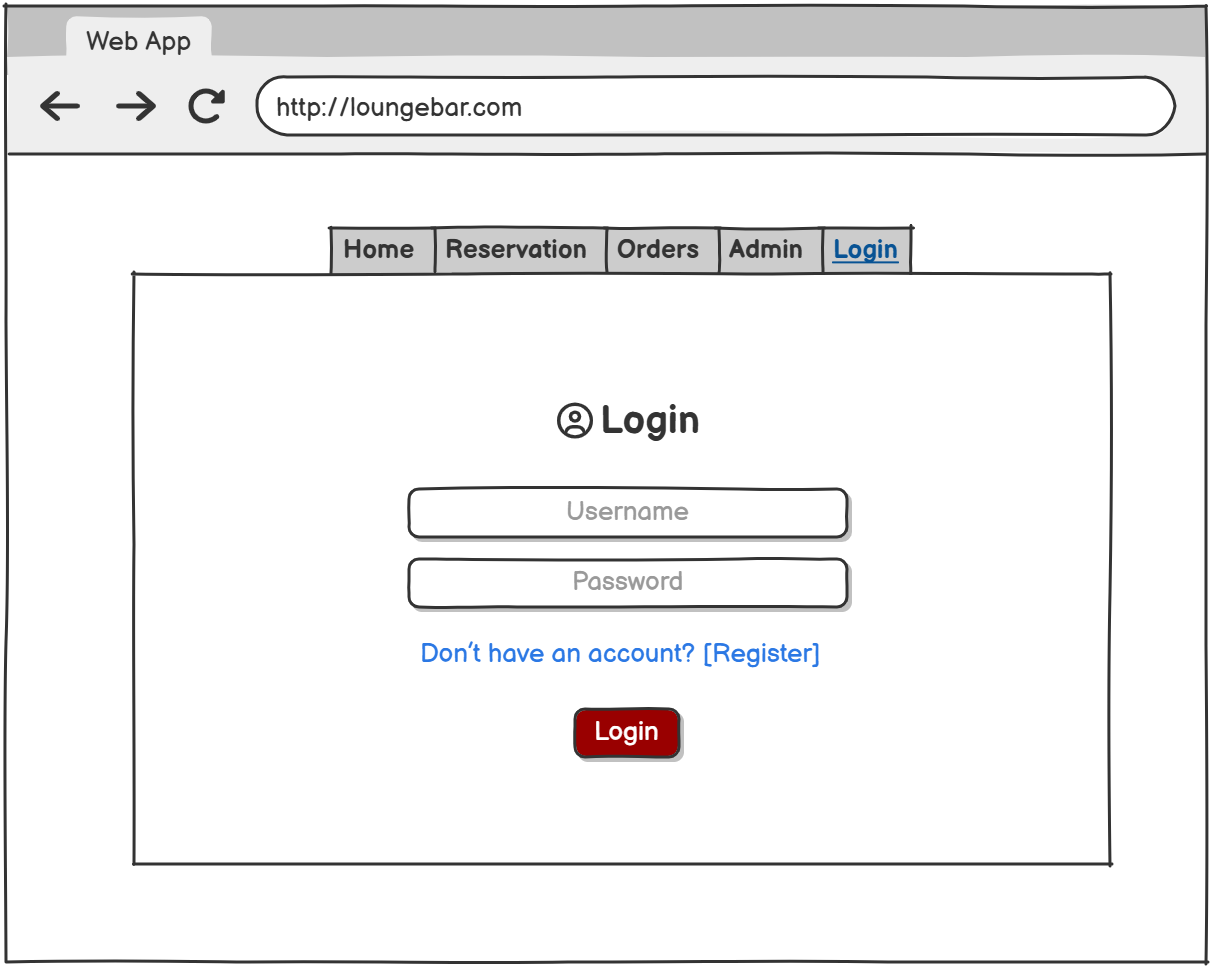
\includegraphics[width=1.1\textwidth]{logos/Login.png}
    \caption{Login page layout}
\end{figure}


\subsection{Reservation Page}

The reservation page allows customers to create a new reservation. It contains a form where users can select the table, specify the reservation date, start time, end time, and the number of people.

The design separates date and time inputs to improve usability and clarity. Once all required information is provided, the user can confirm the reservation through a dedicated action button. The system then processes the request and stores the reservation data in the database.

\begin{figure}[H]
    \centering
        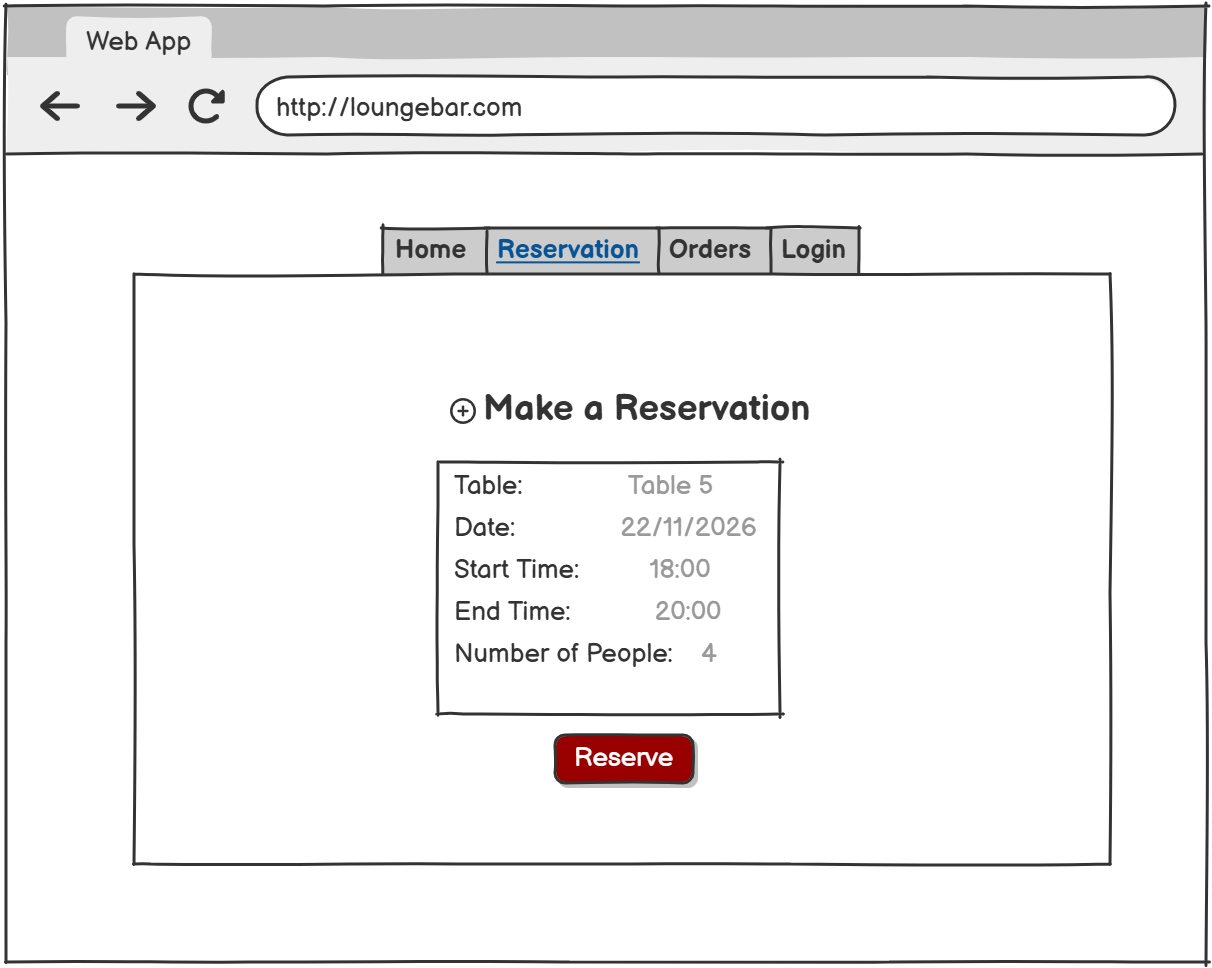
\includegraphics[width=1.1\textwidth]{logos/Reservation.png}
    \caption{Reservation page layout}
\end{figure}


\subsection{Order Management Page}

The order management page is designed for waiters to handle customer orders. It displays key information about the order, including the associated table, the waiter responsible for the service, the date and time, the current status of the order, and the selected payment method.

A table is used to show the list of drinks included in the order along with their quantities. The interface also provides action buttons that allow the waiter to add drinks and update the status of the order during its lifecycle. A confirmation button is also provided to finalize the order once all items have been added.

This page reflects the operational workflow of the system and supports efficient order handling within the lounge bar environment.

\begin{figure}[H]
        \centering
    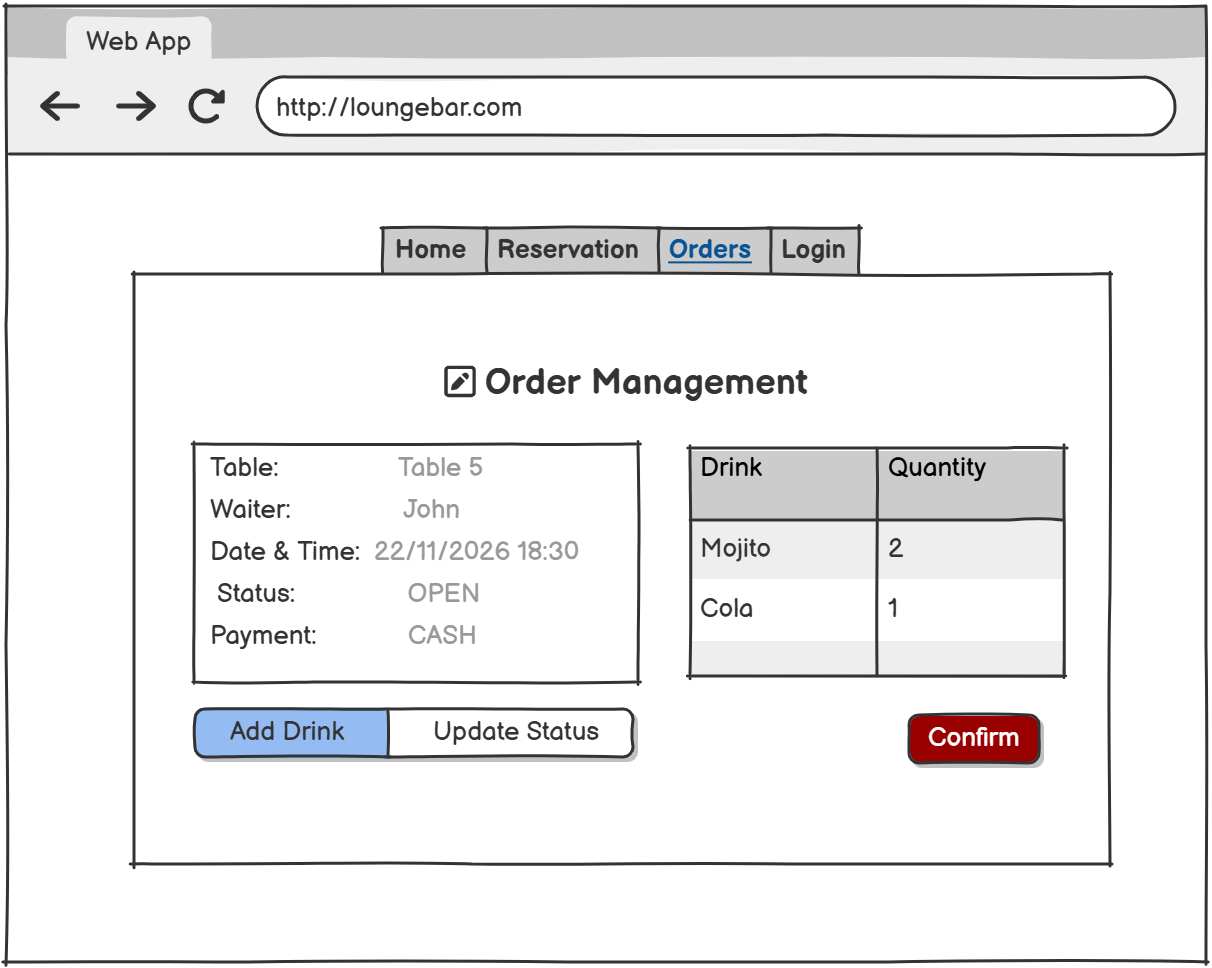
\includegraphics[width=1.1\textwidth]{logos/Order.png}
    \caption{Order management page layout}
\end{figure}













The website is structured into several pages, each responsible for
handling a specific functionality of the lounge bar system. The pages
are designed to provide a clear and user-friendly interface for both
customers and staff.

\begin{itemize}
    \item Homepage: provides general information about the lounge bar and acts as the main entry point of the application. It allows navigation to the main functionalities. Developed using JSP.
    
    \item Login page: allows users to authenticate and access the system according to their role. Developed using JSP.
    
    \item Registration page: allows new users to create an account in the system. Developed using JSP.
    
    \item Reservation page: allows customers to create a new reservation by selecting a table, date, time interval, and number of people. Developed using HTML with support of JavaScript.
    
    \item User profile page: allows users to view and manage their personal information and reservations. Developed using JSP.
    
    \item Order management page: allows waiters to create and manage customer orders, including adding drinks and updating order status. Developed using HTML with support of JavaScript.
    
    \item Drink management page: allows administrators to insert, update, and delete drinks available in the bar. Developed using HTML.
    
    \item Supply management page: allows administrators to manage inventory, including inserting and updating supplies and their available units. Developed using HTML.
    
    \item Shift management page: allows administrators to create shifts and assign waiters to work slots. Developed using HTML.
    
    \item Administration page: allows administrators to manage users and roles within the system. Developed using HTML.
    
    \item Review page: allows customers to submit reviews for waiters, including score and comments. Developed using HTML.
    
    \item Support page: displays feedback messages after completing operations such as insertions, updates, or deletions, providing confirmation to the user.
\end{itemize}





\newpage
\section{BusinessLogicLayer}

\subsection{Class Diagram}

\begin{figure}[H] 
    \centering
    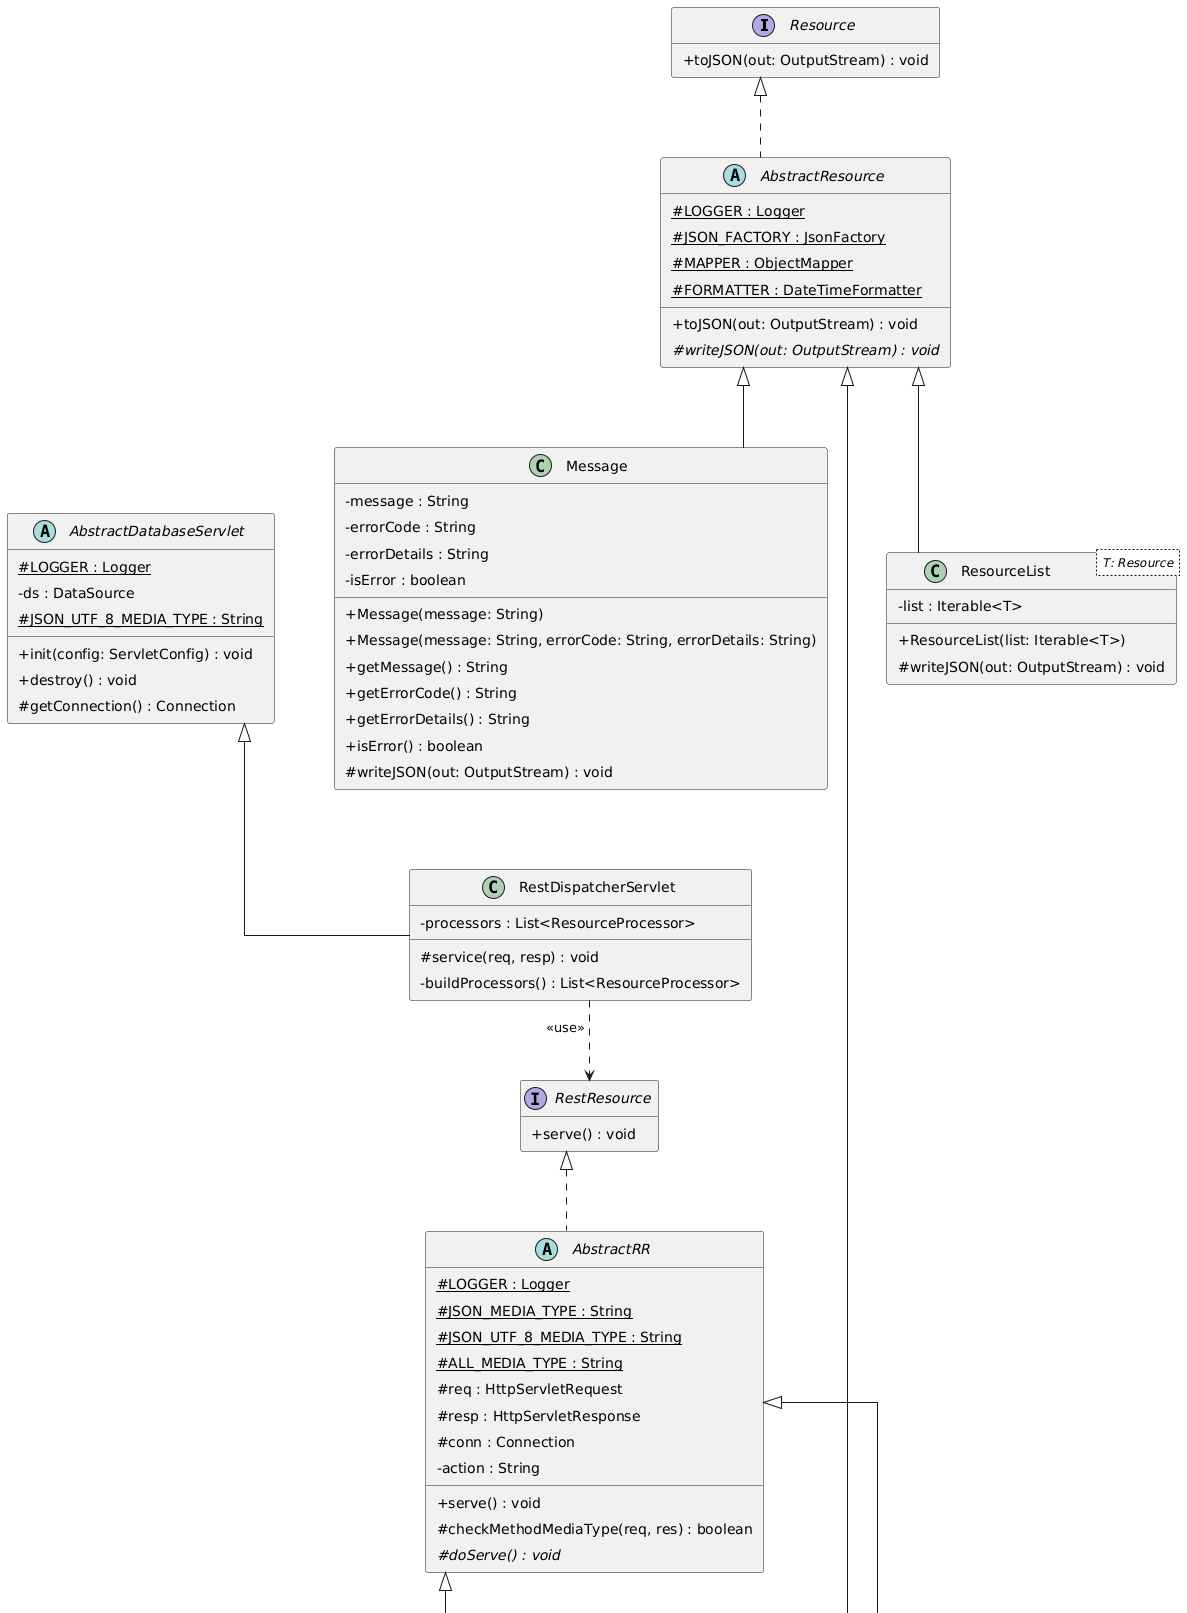
\includegraphics[width=0.8\textwidth]{logos/ReservationRESTWebServiceClassDiagram_part1.png}
\end{figure}

\begin{figure}[H]
    \centering
    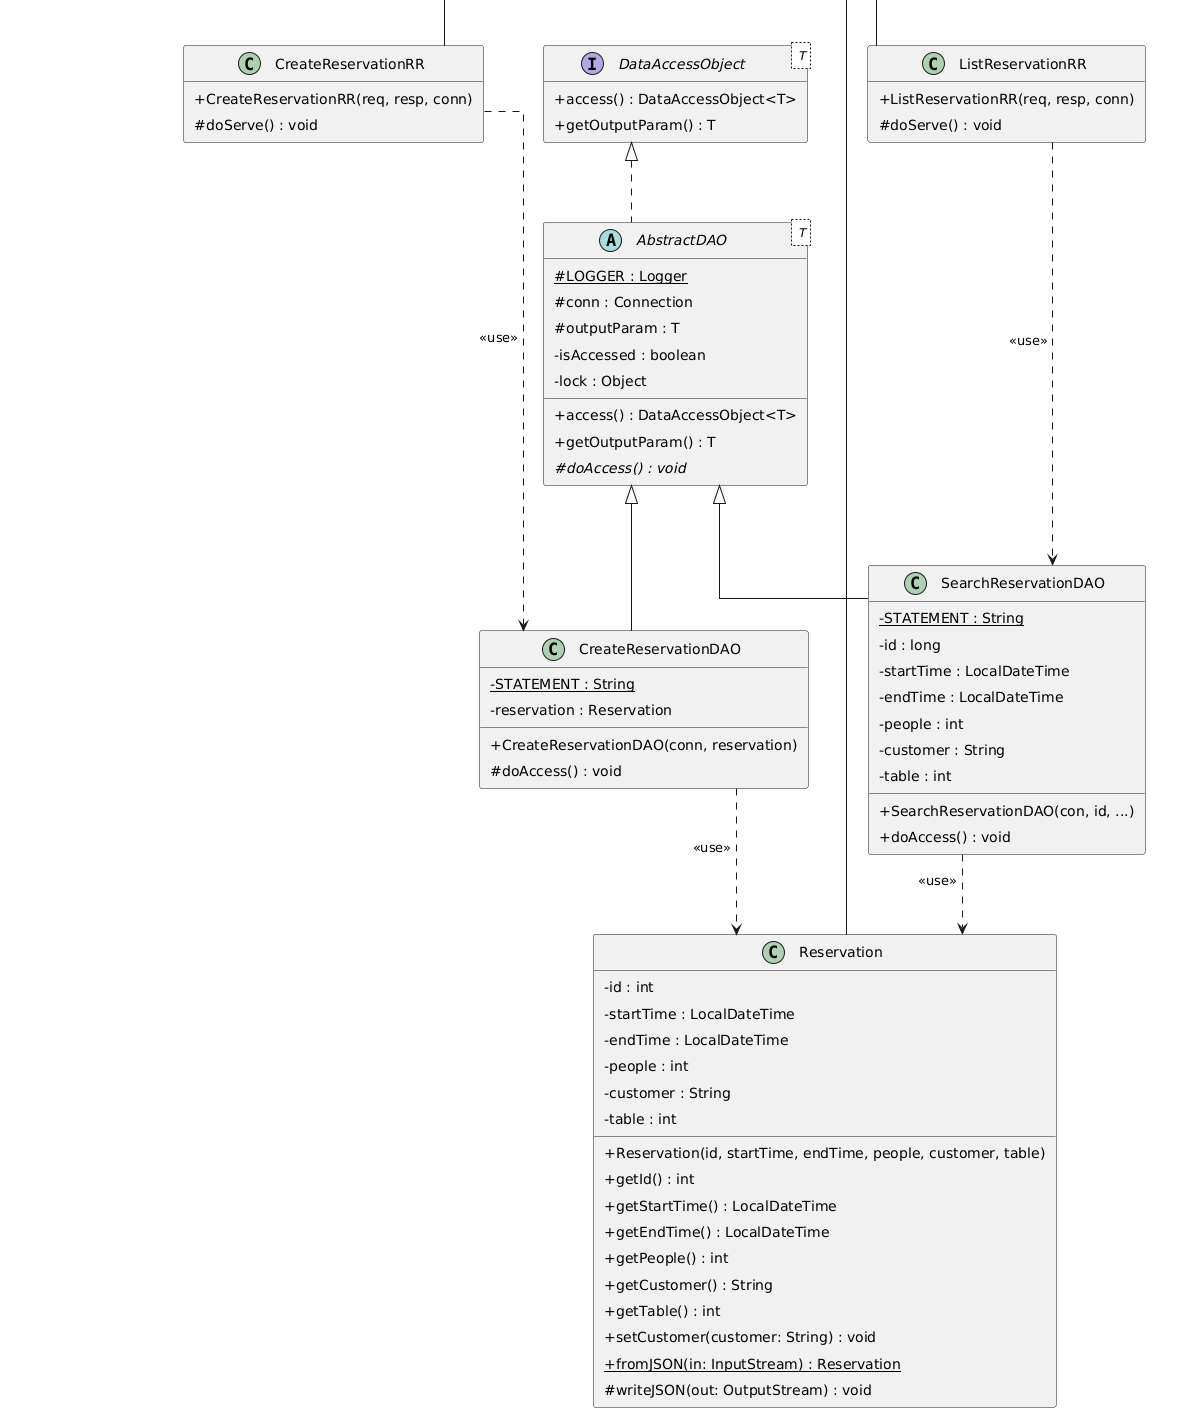
\includegraphics[width=1.0\textwidth]{logos/ReservationRESTWebServiceClassDiagram_part2.png}
    \vspace{0.5cm} 
    \caption{Reservation REST Web Service Class Diagram}
    \label{fig:class_diagram_full}
\end{figure}

The diagram contains only a part of the classes with the main focus on the REST web service for managing Reservations.
There is one servlet - RestDispatcherServlet, which extends AbstractDatabaseServlet to establish the connection to the database. The servlet parses the incoming URL and forwards the request to the handler. Two handlers are shown on the diagram. CreateReservationRR manages the creation of a new reservation, and ListReservationRR handles the search of existing ones. Both extend AbstractRR, which implements the RestResource interface and delegates the logic to the abstract doServe() method.

Also 2 DAO classes support these handlers on the diagram. CreateReservationDAO allows the insertion of a new reservation into the database, and SearchReservationDAO  retrieves reservations from the database. Both extend AbstractDAO, which is delegated to the interaction with the database and defines the doAccess() method. AbstractDAO implements the DataAccessObject interface.

Reservation, Message, and ResourceList<T> are all resource classes that extend AbstractResource. It implements the Resource interface and provides JSON serialization. The Reservation resource holds fields such as start/end time, number of people, customer and table. The Message resource is used to communicate outcomes, such as errors that occurred while handling the resource.


\subsection{Sequence Diagrams}

\begin{figure}[H]
        \centering
        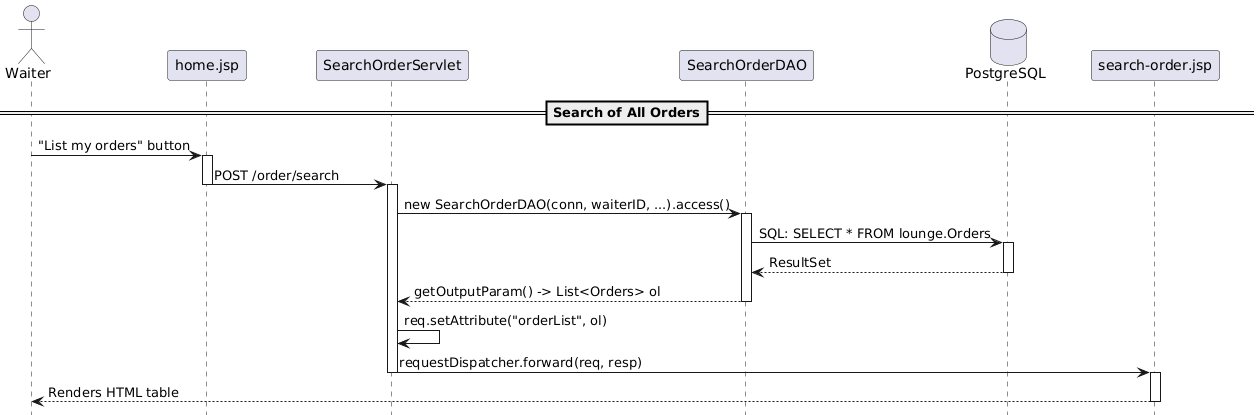
\includegraphics[width=1.0\textwidth]{logos/SearchOrderDiagram.png}
    \caption{Sequence Diagram for Searching Orders}
    \label{fig:search_order}
\end{figure}

This sequence diagram illustrates the flow of the Orders Search operation within the system. The process begins when the Waiter, after being logged in,  interacts with the home.jsp interface. By clicking the "List my orders" button, a POST request is triggered. This request is sent to the web server directed at the URI /order/search/.

Upon receiving the request, the server instantiates the SearchOrderServlet, which returns all the orders of our bar, ordered by the descending time. The servlet then initializes the SearchOrderDAO and invokes its access method. This DAO executes a SELECT query on the specifically the lounge.Orders table of our database to retrieve the orders.

The resulting ResultSet is mapped into an array of Orders objects and returned to the servlet via the getOutputParam method. Finally, the SearchOrderServlet stores this list as a request attribute and performs a forward to the search-order-result.jsp page. This JSP then renders the data, allowing the user to waiter the updated list of orders, including all the details:order ID, date, waiter associated to that order, status of the order, number of the table, pay method and actions to do on the order.

\begin{figure}[H]
        \centering
    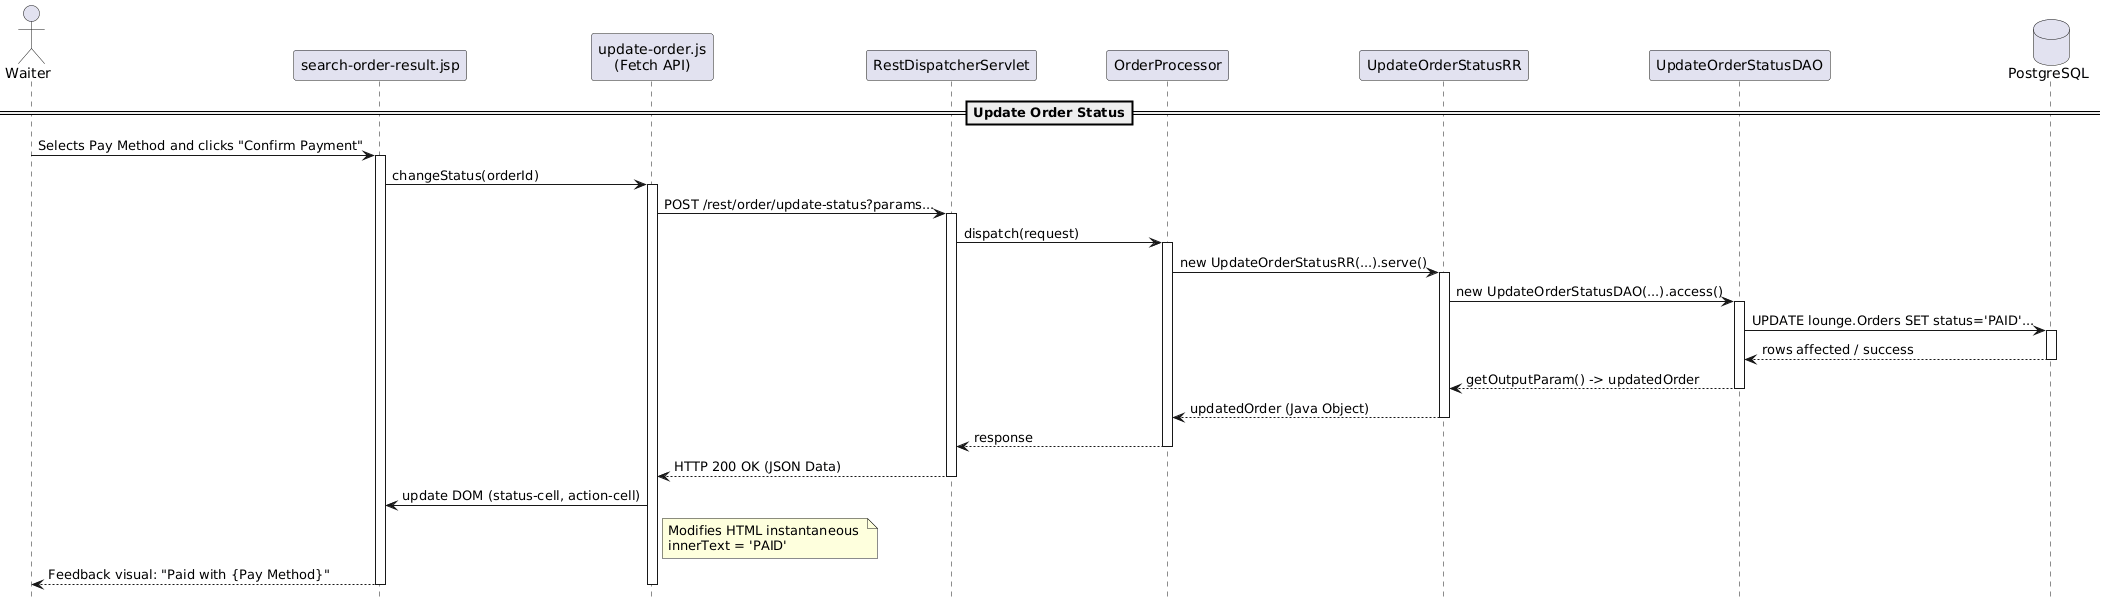
\includegraphics[width=1.0\textwidth]{logos/UpdateOrder.png}
    \caption{Sequence Diagram for Updating Orders}
\end{figure}

This second sequence diagram illustrates the workflow for updating an Order's status and payment method. 
After  searching all the orders of the bar, following the sequence diagram of Figure~\ref{fig:search_order}, the waiter will have a view of all the orders of the bar ordered by time. In this view, he can trigger the Update Order Status by selecting one of the three payment method avalaible (cash, bancomat or debit card) and clicking on the "Confirm Payment" button on the search-order-result.jsp page. This action triggers the changeStatus function within the update-order.js file, which executes a HTTP POST request to the REST endpoint /rest/order/update-status.

The request is intercepted by the RestDispatcherServlet, which dispatches it to the OrderProcessor. The processor then instantiates the UpdateOrderStatusRR REST resource and invokes its serve method. UpdateOrderStatusDAO is initialized to perform an UPDATE statement on the lounge.Orders table in the PostgreSQL database. 

Once the database confirms the operation, the DAO returns the updated order object to the resource, which is then sent back through the processor and dispatcher as a JSON response with an HTTP 200 OK status. Upon receiving this data, the JavaScript logic performs a partial update of the DOM: the status will be updated to 'PAID', the pay method will change to the one selected, and the action cell will be empty for the orders that new instance of the order. All this will be possible without full page reload because of REST. The waiter will see the page immediately changed confirming the transaction.

\subsection{REST API Summary}
The URIs are managed through different access filters. W indicates that only users with the Waiter role can access the endpoint, C signifies that the URI is restricted to Customers. Endpoints labeled as Public are accessible to all users, as they do not require prior authentication (e.g., login and registration pages).

\begin{longtable}{| p{0.20\textwidth} | p{0.12\textwidth} | p{0.43\textwidth} | p{0.10\textwidth} |}
    \caption{Main API Entrypoints} \label{tab:error_codes} \\
    \hline
    \textbf{URI} & \textbf{Method} & \textbf{Description} & \textbf{Filter} \\ \hline
    \endfirsthead
    
    \hline
    \multicolumn{4}{|c|}{Continuation of Table \thetable} \\ \hline
    \textbf{URI} & \textbf{Method} & \textbf{Description} & \textbf{Filter} \\ \hline
    \endhead
    
    \hline
    \endfoot
    
    \hline
    \endlastfoot

    home & GET & Displays the main dashboard page after authentication depending on the user role & W/C \\ \hline
    login & GET & Renders the login form for user authentication & Public \\ \hline
    signup & GET & Renders the registration form to create a new account & Public \\ \hline
    login & POST & Validates credentials and initializes the user session & P \\ \hline
    signup & POST & Processes and stores a new user in the database & Public \\ \hline
    order/search/ & GET & Searches for all the orders of the bar ordered by time & W \\ \hline
    order/add-item/ & POST & Adds a specific drink and its quantity to an existing order & W \\ \hline
    order/update-status/ & POST & Updates order state (PENDING/PAID) and registers the payment method. & W \\ \hline
    shift/create & POST & Records the start of a new work shift for a waiter & W \\ \hline
    supply/create & POST & Registers new inventory or supplies received at the bar & W \\ \hline
    supply/search & POST & Searches the inventory database for specific supplies & W \\ \hline
    review/search-by-waiter & POST & Retrieves reviews for a specific waiter & W \\ \hline
    order/myOrder & POST & Retrieves and displays the current active order for the customer & C \\ \hline
    order/add-items & GET & Loads the interface to select products and add them to an order & W \\ \hline
    supply/search & POST & Searches the inventory database for specific supplies or stock levels. & W \\ \hline
    rest/order/update-status & POST & REST: Updates the order state (e.g., to PAID). & W \\ \hline
    rest/order/add-item & POST & REST: Adds a specific product and quantity to an order without reloading. & W \\ \hline
\end{longtable}
    
    
    

\subsection{REST Error Codes}
The application defines a set of error codes to handle invalid requests
and system errors. Application-specific errors are represented by
negative codes, while HTTP status codes indicate the type of error.


\begin{longtable}{| l | l | p{7cm} |}
    \caption{System and Application Error Codes} \label{tab:error_codes} \\
    \hline
    \textbf{Error Code} & \textbf{HTTP Status} & \textbf{Description} \\ \hline
    \endfirsthead
    \hline
    \multicolumn{3}{|c|}{Continuation of Table \thetable} \\ \hline
    \textbf{Error Code} & \textbf{HTTP Status} & \textbf{Description} \\ \hline
    \endhead
    \hline
    \endfoot
    \hline
    \endlastfoot
    -100 & BAD REQUEST & Missing required parameters \\
    -101 & NOT FOUND & Resource not found \\
    -102 & BAD REQUEST & Invalid input format \\
    -103 & BAD REQUEST & Missing username \\
    -104 & BAD REQUEST & Missing password \\
    -105 & UNAUTHORIZED & Invalid login credentials \\
    -106 & NOT FOUND & User not found \\
    -107 & CONFLICT & Username already exists \\
    -108 & BAD REQUEST & Invalid role \\
    -109 & NOT FOUND & Order not found \\
    -110 & NOT FOUND & Reservation not found \\
    -111 & NOT FOUND & Drink not found \\
    -112 & NOT FOUND & Table not found \\
    -113 & BAD REQUEST & Invalid JSON format \\
    -500 & METHOD NOT ALLOWED & HTTP method not supported \\
    -999 & INTERNAL SERVER ERROR & Unexpected server error \\
\end{longtable}

\subsection{REST API Details}

The following section describes a subset of the REST endpoints
implemented in the lounge bar web application. 

\begin{itemize}

    \item \textbf{User Login}

    The following endpoint allows a user to authenticate in the system.

\begin{itemize}
\item
  \textbf{URL:} \texttt{/login}
\item
  \textbf{Method:} POST
\item
  \textbf{URL Parameters:}\\
  \begin{itemize}
        \item \texttt{role = {string}}: Specifies the user type (e.g., \textit{waiter} or \textit{customer})
    \end{itemize}
  \textbf{Data Parameters (Form Data):}
\end{itemize}
\begin{itemize}
\item \texttt{username = {string}}: The unique identifier or email of the user.
\item \texttt{password = {string}}: The user's credential
\end{itemize}
    
    \item Success Response:
\begin{itemize}
    \item{Code}:\texttt{302 Found}
    \item{Description}: The server validates the credentials and redirects the user to the \texttt{/home} page. A session is created storing the user's email and role.
\end{itemize}

\item Error Response (User Level):
\begin{itemize}
    \item{Code}: \texttt{401 Unauthorized}
    \item{Description}: Occurs if the credentials are invalid or the role does not match. The user is redirected back to the login page with an error message.
\end{itemize}

    \item Error Response (Server Level):
\begin{itemize}
    \item{Code}: \texttt{500 Internal Server Error}
    \item{Description}: Triggered by a \texttt{SQLException} or \texttt{NamingException} when the database is unreachable. 
    \item{Content}: \texttt{\{"error": \{"code": -999, "message": "Internal Error"\}\}}
\end{itemize}


    
   
    \item \textbf{Reservation Creation}

    Allows a customer to create a reservation for a table.
    
    \begin{itemize}
    \item
      \textbf{URL:} \texttt{/rest/reservation/create}
    \item
      \textbf{Method:} \texttt{POST}
    \item
      \textbf{URL Parameters:}\\
      No parameters are required in the URL.

    \item \textbf{Data Parameters (JSON):}
    \begin{itemize}
        \item \texttt{tableNumber = \{integer\}}: The identifier of the selected table.
        \item \texttt{user\_customerID = \{string\}}: The unique username of the customer.
        \item \texttt{start\_time = \{time\}}: The expected arrival time.
        \item \texttt{end\_time = \{time\}}: The expected departure time.
        \item \texttt{n\_people = \{integer\}}: Total number of guests.
    \end{itemize}

\item Success Response:
    \begin{itemize}
        \item{Code}: \texttt{201 Created}
        \item{Content}: \texttt{\{"message": "Reservation successfully created", "id": \{integer\}\}}
        \item {When}: All validation checks pass and the table is available for the requested time slot.
    \end{itemize}

    \item Error Response (Business Level):
    \begin{itemize}
        \item{Code}: \texttt{409 Conflict}
        \item{When}: The selected table is already reserved for the specified date and time.
    \end{itemize}

    \item Error Response (Server Level):
    \begin{itemize}
        \item{Code}: \texttt{500 Internal Server Error}
        \item{Content}: \texttt{\{"error": \{"code": -999, "message": "Database error"\}\}}
        \item{When}: A \texttt{SQLException} occurs during the insertion process.
    \end{itemize}
\end{itemize}





\section{Contributions}



\begin{description}[style=multiline, leftmargin=3cm, font=\bfseries]
    
    \item[Bruzzese Fulvio] Setting structure of the project, creation of several Java classes, creation of several DAOs while fixing database errors, creation of several Servlets with respective .jsp and its functionalities. Created REST functionalities such as CreateReservation or CreateReview with respective .jsp and .js. Creation of README document
    
    \item[Foffano Claudia] Setting structure of the project, creation Java classes, creation of several DAOs while fixing database errors. Tried to resolve some errors of .jsp and .js files. Arranged the entire document and described the main functionalities.
    
    \item[Halawani Sondos] Shared first draft of the documentation and mock-ups

    \item[Iacobet Ecaterina] Setting up the database based on the FDB project before, modifying the ER schema, creation Java classes, creation of several DAOs while fixing database errors, creation of several Servlets with respective .jsp and its functionalities. Implemented REST functionalities such as ListWaitersRR with its respective .jsp and .js files. Class diagrams for the document and described the main functionalities.

    
    \item[Núñez Casal Luis Ignacio] Setting structure of the project, creation Java classes, creation of several DAOs while fixing database errors, creation of several Servlets with respective .jsp and its functionalities. Created REST functionalities such as UpdateOrderStatus with respective .jsp and .js. Sequence diagrams of the document and changes in APIs sections
    

\end{description}


\end{document}
